% ============================================================
%  sec07.tex —— §7 椭圆曲线镜像对称的图示（原文 pp.38–44）
%  原文：Homological Mirror Symmetry for Elliptic Curves
%  外部交叉引用均按 GUIDE §6.5 的“原文编号” key：
%    thm:6.1, thm:6.4, thm:4.2, prop:2.5, thm:3.2,
%    subsec:maslov (4.3.2), subsec:6.3 (原文 “compare section 6.3”)
%  本节自身带编号的定理类：prop:7.1, thm:7.2, thm:7.3；
%  7.3 中原文不带编号的 Lemma 用 lemma*（不占计数，以保证 thm:7.3 编号正确）。
% ============================================================

\section{椭圆曲线镜像对称的图示}
\label{sec:illus}

\begin{keytakeaways}
  \item \textbf{物理/几何图像}：$T$ 中斜率为 $m/n$ 的测地圆在镜像下对应 $E$ 上秩 $n$、次数 $m$ 的向量丛；镜像曲线的方程由 $A$、$B$ 两条标准经线之间的多边形计数完全确定。
  \item \textbf{数学工具}：扭变函子 $T_B^{3n}$ 作用下的 Hom 空间给出射影坐标环，theta 级数 $A_i$、$B_i$ 给出结构常数，$j$-不变量由 Hesse 型三次方程的参数 $z$ 算出。
  \item \textbf{核心结论}：镜像曲线是 $\Lambda_t$ 上的光滑平面三次曲线，其 $j$-不变量等于经典 $j(q)$ 的 Laurent 展开（定理~\ref{thm:7.2}）；并且对任意 $C\in\Fuk(T)$ 有 $h(C)=k(\psi(C))$（定理~\ref{thm:7.3}）。
\end{keytakeaways}

本节我们打算收获此前为证明定理~\ref{thm:6.1} 与~\ref{thm:6.4} 所付出的全部努力。回忆我们已在其中证明：存在某个三次曲线 $E$，以及拟等价
\[
\psi\colon D^\pi\Fuk(T)\longrightarrow \Dinf(E).
\]
它由 $\psi(A)=\cO$ 与 $\psi(B)=\cO/P$ 确定，其中 $A$、$B$ 是标准经线（meridians）。

然而，我们并不知道 $E$ 是哪条曲线，甚至不知道它是否光滑。我们在第~\ref{subsec:determination}~小节解决这个问题。事实上，定理~\ref{thm:6.4} 还包含了确定 $E$ 的方法：从对应 $\cO$ 与 $\cO/P$ 的两条标准经线 $A$、$B$ 出发，考虑环
\[
S=\bigoplus_{n\ge 0}\Hom_{H^0D^\pi\Fuk(T)}\bigl(A,\,T_B^{3n}(A)\bigr).
\]
这是 $E$ 的射影坐标环。利用一些显式的多边形计数，我们可以求出 $E$ 的定义方程、验证它光滑，并计算其 $j$-不变量。

% [Tutor Note: 这里出现的指数是 $3n$ 而不是 $n$：$S$ 的第 $n$ 个分次片 $S_n=\Hom(A,T_B^{3n}(A))$ 的维数为 $3n$（$S_1$ 维数 3、$S_2$ 维数 6、$S_3$ 维数 9），恰好等于 $h^0(\cO_E(3n))=3n$。可把这个维数作为核对“$T_B^{3n}$ 对应 $\cO_E(3n)$ 的 Serre 扭转”这一对应关系的独立校验；若把指数误读成 $n$，则 $S_1$ 只有一维，无法给出三次曲线的三个齐次坐标。]

完成这些后，我们更细致地研究镜像对应 $\psi$。在第~\ref{subsec:rank-slope}~小节，我们定义向量丛的秩与斜率，并说明 $T$ 中斜率为 $m/n$ 的测地圆 $C$ 如何对应到镜像对应下它在 $\Dinf(E)$ 中所代表的向量丛的秩与斜率。

观察到群 $SL_2(\ZZ)$ 自然地作用在 $T$ 上，从而它（或更确切地说，它的中心扩张）作用在 $\Fuk(T)$ 上。由镜像对应，$\Dinf(E)$ 上必存在相应的作用。在第~\ref{subsec:braid}~小节我们构造这一作用，并用它证明上一小节草拟的秩与斜率对应。

\subsection{镜像曲线的确定}
\label{subsec:determination}

我们现在执行上面草拟的方法。为此，我们在 $T$ 的万有覆盖 $\RR^2$ 中工作。注意 $\rho(x,y)=(x,y+3x)$ 是 $\tau_B^3$ 的一个模型。令 $L_i=\rho^i(A)$。

% [Tutor Note: $\rho$ 是三次 Dehn 扭转 $\tau_B^3$ 在万有覆盖上的仿射模型，而不是 $\tau_B$ 本身——这正是“指数 3”的来源。核对时可在 $\RR^2/\ZZ^2$ 上看 $\rho$ 的线性部分 $\left(\begin{smallmatrix}1&0\\3&1\end{smallmatrix}\right)$：它的幂 $\rho^i$ 给出斜率为 $3i$ 的直线 $L_i$，即 $L_i=\rho^i(A)$。若误把 $\rho$ 当作一次扭转，则 $L_1$ 会是斜率为 1 的直线，与 $X_i=(i/3,0)$ 等交点坐标全部对不上。]

我们必须找到 $S_1=\Hom(A,L_1)$ 的（三个）生成元，以及它们在 $S_3=\Hom(A,L_3)$ 中满足的一个三次关系。为此，令 $X_i=(i/3,0)$（$i=0,1,2$），$Y_i=(i/6,0)$（$i=0,\ldots,5$），$Z_i=(i/9,0)$（$i=0,\ldots,8$）。这里以及别处，指标都按适当的 $n$ 作“$(\mathrm{mod}\ n)$”理解（例如对 $X_i$ 取 $n=3$）。注意 $\Hom(A,L_i)$ 是集中位于 $0$ 次、维数为 $3i$ 的分次向量空间。事实上，$X_i\in\Hom(A,L_1)$、$Y_i\in\Hom(A,L_2)$、$Z_i\in\Hom(A,L_3)$ 分别是这些向量空间（即交点）的自然生成元。

% [Tutor Note: 三组交点的分母不同并非笔误：$A$ 与 $L_i$（斜率 $3i$ 的直线）在基本域内恰有 $3i$ 个交点，所以 $X_i$ 分母为 3（3 个点）、$Y_i$ 分母为 6（6 个点）、$Z_i$ 分母为 9（9 个点）。所有 Hom 空间都集中在 0 次（无分次移位），因此后面三次关系的系数是纯数（theta 级数），不涉及 Koszul 符号。]

于是，我们需要做的是：把 $X_i$ 的十个三次单项式用 $\Hom(A,L_2)$ 的九个基元素 $Z_j$ 表示出来。这里必须回忆，$S$ 上的环结构是“经由 $\rho$”产生的。例如 $X_1X_2$ 指的是 $m_2(\rho(X_1),X_2)\in\Hom(A,L_2)$，其中我们把 $\rho(X_1)\in\Hom(\rho(A),\rho(L_1))=\Hom(L_1,L_2)$ 计算在内。

% [Tutor Note: 原文此处作“nine basis elements $Z_j$ of $\Hom(A,L_2)$”，但按上文 $Z_j\in\Hom(A,L_3)$、且 $\dim\Hom(A,L_3)=9$，这里应为 $\Hom(A,L_3)$。译文保留原文写法，见汇报中的原文疑误清单。]
% [Tutor Note: 这个“经由 $\rho$”的乘法是本节最容易出错的地方：复合 $m_2(\rho(X_1),X_2)$ 要求第一个因子的起点先被 $\rho$ 搬到 $L_1$，因此单调的“交换环”直觉在此失效，$A_{i-j}$、$B_{2j-i}$ 中指标的正负号与偏移（$+3$、$+6$、$+12$）都来自这个扭曲。算三次单项式前，务必先用已知的交换性、结合性核对 $X_iX_j=X_jX_i$。]

因此我们真正想做的是：先把 $X_i$ 的六个二次单项式用 $Y_j$ 表示，再由此算出三次单项式。这里我们用到了已知的事实：$S$ 必须是交换且结合的。

让我们看一个例子。假设要用 $Y_j$ 表示 $X_0^2$。于是我们要找顶点为 $X_0$、$\rho(X_0)=X_0$ 以及某个 $Y_j$ 的三角形。考虑图~\ref{fig:triangles}。

% [Tutor Note: 原文此处引用“figure 7.1”，但原书该图的实际编号是 Figure 3（第 40 页，本译本为图~\ref{fig:triangles}）。这是原文自身的编号不一致（正文用章节式编号，图题用全文连续编号）；译文正文按实际图编号引用，不再保留“7.1”这一不存在的图号。]

该图显示万有覆盖，其中所有点与曲线（直线）都无限次重复。图中用阴影标出的是我们要找的两个三角形 $F$ 与 $G$。容易看出，其余所有对 $X_0^2$ 有贡献的三角形都是这两个三角形的平移与伸缩。由此可得 $X_0^2=A_0Y_0+A_3Y_3$。我们来确定 $A_3$。这意味着要数 $F$ 的伸缩。容易看出，它们由整数 $n\in\ZZ$ 标号，顶点为 $(0,0)$、$(2n+1,6n+3)$ 与 $(0,n+1/2)$。图中所示的三角形 $F$ 对应 $n=0$。对应 $n$ 的三角形面积为
\[
\frac12\Bigl(n+\frac12\Bigr)(6n+3)=3\Bigl(n+\frac12\Bigr)^2 .
\]
因此
\[
A_3=\sum_{n\in\ZZ} t^{\,3(n+\frac12)^2}.
\]

% [Tutor Note: 这里的 $t$ 是 Novikov 变量，单项式 $t^{\text{面积}}$ 记录三角形的辛面积（相对于基本域面积归一化）。面积公式 $3(n+1/2)^2$ 是“底 $\times$ 高 $/2$”：竖直边长为 $n+1/2$、水平宽为 $6n+3$。面积对 $n\to -n-1$ 对称，这正是 theta 级数出现的原因；同时它解释了为什么 $A_3$ 只含半整数平移的项。]

这是一个经典的 theta 级数。事实证明，我们必须做的所有三角形计数都给出这类级数。Zaslow \cite{ref24} 详细完成了这些计数。他的结果可概括如下。记
\[
A_i=\sum_{n\in\ZZ} t^{\,3(n+\frac{i}{6})^2},
\qquad
B_i=\sum_{n\in\ZZ} t^{\,9(n+\frac{i}{18})^2}.
\]
则
\[
\begin{aligned}
X_iX_j &= A_{i-j}Y_{i+j}+A_{i-j+3}Y_{i+j+3},\\
Y_iX_j &= B_{2j-i}Z_{i+j}+B_{2j-i+6}Z_{i+j+3}+B_{2j-i+12}Z_{i+j+6}.
\end{aligned}
\]

由此，求出三次单项式之间的线性关系完全是例行公事，尽管相当繁琐。由它可以计算镜像的 $j$-不变量。结果如下。

\begin{proposition}[Zaslow]\label{prop:7.1}
令
\[
u=A_2B_0+A_1B_9,\qquad p=A_0B_0+A_3B_9,\qquad q=A_0B_6+A_3B_3,\qquad z=\frac{2q+p}{3u}.
\]
则 $X_i$ 满足的三次关系为
\[
X_0^3+X_1^3+X_2^3-3z\,X_0X_1X_2=0.
\]
这是一条光滑三次曲线，其 $j$-不变量为
\[
j_{\Fuk}=-27\,\frac{z^3(z^3+8)^3}{(1-z^3)^3}.
\]
\end{proposition}

% [Tutor Note: 作者写“working out the linear relation ... is entirely routine”，省略的实质是：$S_3=\Hom(A,L_3)$ 是 9 维空间，而 $X_i$ 的三次单项式有 $\binom{5}{3}=10$ 个，故必存在唯一（差一个标量）的线性关系；$S$ 的交换性把它对称化为 $X_0^3+X_1^3+X_2^3-3zX_0X_1X_2=0$，参数 $z$ 由代入 $A_i,B_i$ 的显式 theta 级数确定。实际计算顺序是：先用 $A_i$ 把六个二次单项式写成 $Y_j$ 的组合，再用 $B_i$ 把 $Y_jX_k$ 写成 $Z_l$ 的组合，最后消去 $Y$、$Z$。]
% [Tutor Note: 核对 $j$-不变量时注意参数约定：Hesse 型三次曲线 $X^3+Y^3+Z^3-3zXYZ=0$ 的 $j$-不变量为 $-27z^3(z^3+8)^3/(1-z^3)^3$；经典模 lambda 函数公式是 $j=256(1-\lambda+\lambda^2)^3/[\lambda^2(1-\lambda)^2]$。$z$ 与 $\lambda$ 之间是分式线性变换（Hesse 参数与 Legendre 参数），不可直接令 $z=\lambda$ 或 $z^3=\lambda$。建议用两个特殊值锚定归一化：$j(i)=1728$，$j(e^{2\pi i/3})=0$。另注意原文在此把 $j$-不变量记作 $j_{\Fuk}$ 以区别于经典 $j$。]

这完全回答了本小节提出的问题。此外，Zaslow 观察到，在我们呈现镜像对称的方式下，出现了一个小小的奇迹。考虑上半平面中的 $\tau$，以及复环面 $E_\tau=\CC/\ZZ\oplus\tau\ZZ$。这是一条椭圆曲线，其 $j$-不变量是经典函数。它通常用 $q=e^{2\pi i\tau}$ 写出，因为此时它具有整系数的 Laurent 级数展开 \cite{ref13}：
\[
j(q)=\frac1q+744+196884q+\ldots
\]

% [Tutor Note: 原文排印为 $E_\tau=\CC/\ZZ\oplus\tau\ZZ$；按数学含义应读作 $\CC/(\ZZ\oplus\tau\ZZ)$（斜杠只作用于整个格）。这是原文的一处排印歧义，译文保留原式并在此标注。]
% [Tutor Note: 指数约定必须核对：$q=e^{2\pi i\tau}$（不是 $e^{\pi i\tau}$），于是 $j(q)=q^{-1}+744+196884q+\cdots$，其中 196884 是 Monster 表示维数（McKay 观察）。若换成 $Q=e^{\pi i\tau}$ 的约定，展开式会变成 $Q^{-2}+\cdots$，系数完全不同。后文镜像映射把形式变量 $t$ 与 $q$ 等同起来，这个替换的逐阶验证正是定理~\ref{thm:7.2} 的内容。]

% 图 3 原位于第 40 页顶部；正文在 7.1 开头引用它（原文误作“figure 7.1”）。fig3.pdf 已按整幅图重新裁剪。
\begin{figure}[htbp]
  \centering
  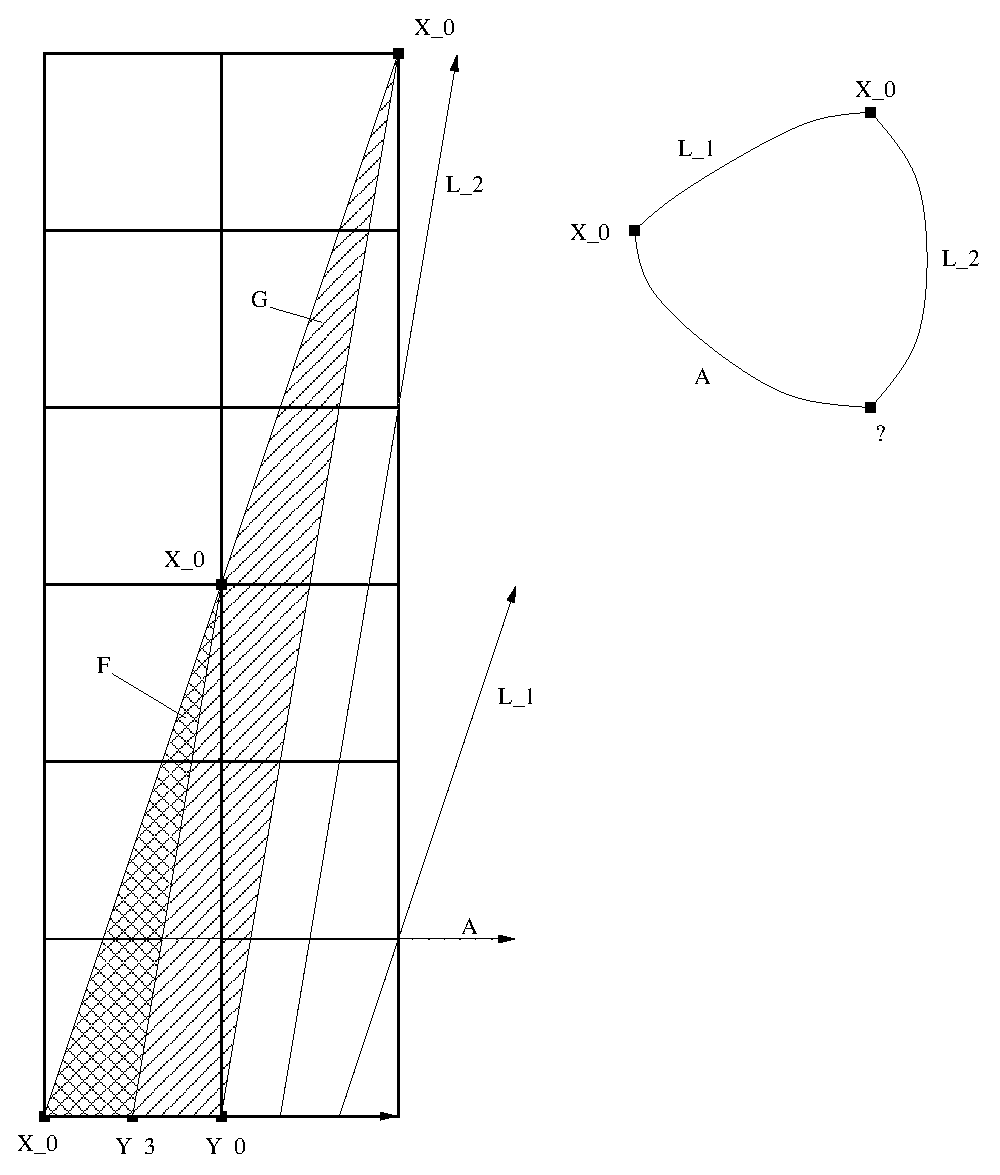
\includegraphics[width=0.95\linewidth]{figures/fig3.pdf}
  \caption{对 $X_0^2$ 有贡献的部分三角形。左图为 $T$ 的万有覆盖：网格、直线 $A$、$L_1$、$L_2$，标记点 $X_0$、$Y_0$、$Y_3$，以及用阴影标出的三角形 $F$ 与 $G$；右图为环面上由曲线段 $A$、$L_1$、$L_2$ 围成的三角形，两个顶点标为 $X_0$，第三个顶点标为“？”。（原文 Figure 3，第 40 页）}
  \label{fig:triangles}
\end{figure}

\begin{theorem}\label{thm:7.2}
$T$ 的镜像曲线是 $\Lambda_t$ 上的光滑平面三次曲线，其 $j$-不变量 $j$ 由经典 $j(t)$ 函数的 Laurent 展开给出。
\end{theorem}

% [Tutor Note: 这个定理的“证明”被作者略去了。作者在下一段说原则上可以证明 $j_{\Fuk}(t)$ 是模函数、再比较有限维空间中的前几项；实际需要验证的是 $j_{\Fuk}$ 在 $SL_2(\ZZ)$（或某个同余子群）下的变换性质，这是 Zaslow \cite{ref24} 的 theta 级数计算的核心，属于“非平凡”的部分。作者随后用 $O(q^4)$ 的逐阶验证代替证明，这一点务必在引用定理时说明。]

原则上，可以通过证明 $j_{\Fuk}(t)$ 是模函数、再计算级数展开的前几项来证明这一点（因为模函数空间是有限维的）。然而，这相当不平凡。我们转而满足于逐阶验证该断言，想要多少项就验证多少项（这当然不是证明，但仍颇具说服力）：附录中图~\ref{fig:series-py} 的 Python 脚本 \texttt{series.py} 可用于计算 $j_{\Fuk}(t)$ 的级数展开到任意所需阶数。它通过暴力计算进行，即先把 $j_{\Fuk}(t)$ 中出现的 theta 函数计算到足够高的阶数，然后求逆并相乘。我们已用它验证该断言直到 $O(q^4)$。

\subsubsection*{$\CC$ 上的镜像对称}

一个有趣的观察是：给定上半平面中的一个复数 $q$，可以构造一个 $A_\infty$-范畴 $\Fuk_q(T)$，它由 $\Fuk(T)$ 通过把 $t$“替换”为 $q$ 得到。也就是说，定义中相应的级数实际上收敛。上述结果于是表明：若 $E$ 是 $\CC$ 上一条 $j$-不变量为 $j(q)$（对某个特定的 $q\in\CC$）的椭圆曲线，则 $\Dinf(X)$ 与 $D^\pi\Fuk_q(T)$ 拟等价。因此，在 $\CC$ 上，我们为所有椭圆曲线找到了镜像。

% [Tutor Note: 原文此处有两处容易误导的地方。其一，“given a complex number $q$ in the upper half plane”中的 $q$ 应为模参数 $\tau\in\mathbb{H}$（$q=e^{2\pi i\tau}$ 并不在上半平面）；这是原文的笔误，译文保留原词并在此标注。其二，结论中的 $\Dinf(X)$ 按上下文应为 $\Dinf(E)$（$E$ 才是被镜像的椭圆曲线，本节从未定义过 $X$）；同样保留原文并标注。理解时按“$\tau\in\mathbb{H}$，$\Dinf(E)\simeq D^\pi\Fuk_q(T)$”读即可。]

\subsection{图示的镜像对称：向量丛的秩与斜率}
\label{subsec:rank-slope}

我们的镜像对称证明相当抽象。特别地，确定嵌入圆 $C\in\Fuk(T)$ 在镜像对应下的像 $\psi(C)$ 绝非平凡。这里我们至少希望描述 $\psi(C)$ 是何种对象。事实上，可以证明它总是（某个平移下的）局部自由层或摩天楼层，因此一个非常自然的问题是：$\psi(C)$ 具有怎样的秩与第一陈类。这就是本小节要处理的问题。

设 $\cA$ 是三角 $A_\infty$-范畴，$B$ 是阿贝尔群。若对 $\cA$ 中任意态射 $f\colon X\to Y$ 都有
\[
0=e(X)-e(Y)+e(\operatorname{cone}(f)),
\]
则称映射 $e\colon\Ob(\cA)\to B$ 为欧拉示性数（或加性函数）。显然，$e$ 由它在 $\cA$ 的任意一组生成元（而不必是分裂生成元）上的取值确定。例如，若 $\cA=\Dinf(X)$、$X$ 是光滑射影簇，则 $e$ 由它在向量丛上的取值确定（由定理~\ref{thm:3.2}，这些向量丛是生成元）。

% [Tutor Note: 欧拉示性数的定义等价于“在正合三角形上可加”：由 $X\to Y\to\operatorname{cone}(f)\to$ 得 $e(X)-e(Y)+e(\operatorname{cone}f)=0$，故 $e$ 是三角范畴上的加性函数。注意“生成元”与“分裂生成元（split-generators）”的区别：这里只要求生成元，是因为 $e$ 在三角范畴上可加、自动沿分裂闭包延拓；若换成一般的加法不变量，可能只由分裂生成元决定。此外 $e$ 必在平移下变号：$e(X[1])=-e(X)$。]

设 $\cA$ 是 $k$ 上的三角 $A_\infty$-范畴，$X\in\cA$ 具有有限上同调维数，即：对任意 $Y\in\cA$ 存在 $n$，使得对所有 $|r|>n$ 有 $H^r\Hom_{\cA}(X,Y)=0$，并且对所有 $r$ 有 $\dim_k H^r\Hom_{\cA}(X,Y)<\infty$。此时
\[
e(Y)=\sum_i(-1)^i\dim_k H^i\Hom_{\cA}(X,Y)=:\chi\bigl(H^*\Hom(X,Y)\bigr)
\]
是 $\cA$ 上的欧拉示性数。这来自 $H^0\cA$ 是三角范畴这一事实。对 $\Hom(\bullet,X)$ 有类似结果。

现在设 $X$ 是光滑射影簇，$P\in X$ 是闭点。我们在 $\Dinf(X)$ 上定义两个欧拉示性数，称为秩与斜率：
\[
\operatorname{rk}(\cF)=\chi\bigl(\Ext^*(\cF,\cO_X/P)\bigr),
\qquad
\operatorname{sl}(\cF)=\chi\bigl(\Ext^*(\cO,\cF)\bigr)=\chi\bigl(H^*(X,\cF)\bigr).
\]
容易看出，对局部自由层，这个秩的定义与通常的定义一致，从而特别地不依赖于 $P$ 的选取。又若 $X$ 是椭圆曲线、$\cL$ 是线丛，则由 Riemann--Roch 定理与 Serre 对偶，$\cL$ 的斜率等于其次数（即第一陈类）。\footnote{可以证明第一陈类 $c_1$ 也是欧拉示性数。若 $X$ 不是椭圆曲线，这或许是比我们的定义更好的斜率定义。由于我们只处理椭圆曲线，我们将忽略这个问题。}

% [Tutor Note: 秩的定义用 $\cO_X/P$（摩天楼层）而不是 $\cO_X$：$\chi(\Ext^*(\cF,\cO_X/P))$ 数的是 $\cF$ 在 $P$ 处的纤维维数，对局部自由层恰好等于秩，且与 $P$ 无关；斜率则用 $\cO$ 配对，$\chi(\Ext^*(\cO,\cF))=\chi(H^*(X,\cF))$，对线丛由 Hirzebruch--Riemann--Roch 得 $\deg$。核对时注意 $\Ext^*$ 指全 Ext 复形（带分次），$\chi$ 是交错和而不是 $\dim\Hom$。]

当然，我们可以把这两个欧拉示性数组合起来，得到映射
\[
k\colon \Dinf(E)\to\ZZ^2,\qquad \cF\mapsto\bigl(\operatorname{sl}(\cF),\operatorname{rk}(\cF)\bigr).
\]
在镜像对称下，它对应映射 $k'\colon\Fuk(T)\to\ZZ^2$，由相同的公式定义。

还有另一个来自几何的、形式类似的映射，从 $\Fuk(T)$ 出发。即回忆 $\Fuk(T)$ 的对象（不是 $D^\pi\Fuk(T)$ 的对象）由带额外数据的嵌入圆表示。于是我们有映射
\[
h\colon \Fuk(T)\to H_2(T)\simeq\ZZ^2.
\]
具体地，若曲线 $C$ 在 $T$ 的万有覆盖中由斜率为 $m/n$ 的直线表示（并且“朝右”定向），其中分式已约至最简且 $n>0$，则 $h(C)=(m,n)$。这就解释了“斜率”一词。

% [Tutor Note: 几何直观：$h$ 把拉格朗日圆周送到它的同调类；在万有覆盖中取斜率为 $m/n$ 的直线，$m,n$ 就是它相对于标准经线 $A,B$ 的同调系数。镜像一侧的 $(\operatorname{sl},\operatorname{rk})=(m,n)$ 意味着“斜率 $m/n$”在代数侧应读作“次数/秩”。作者把 $h$ 与 $k'$ 都取成二元组，正是为了让 $SL_2(\ZZ)$ 的线性作用两边一致；注意 $k$ 的分量次序是（斜率，秩），与 $h$ 的（$m,n$）次序相同，不要颠倒。]
% [Tutor Note: “oriented to the right”与 $n>0$ 的约定是固定符号的关键：同一条无向直线有两种定向，取 $n>0$ 的定向消除这个二义性，否则 $h(C)$ 会差一个整体符号 $(m,n)\mapsto(-m,-n)$。$SL_2(\ZZ)$ 作用正是以这种方式把不同的 $(m,n)$ 联系起来。]

我们断言 $h=k'$（在有定义处）。这用手检查并不特别困难。这里我们验证 $h(C_x)=k'(C_x)$，其中 $C_x$ 是对应于平行于 $A$ 的直线
\[
\{(t,x)\mid t\in[0,1]\}
\]
的曲线。一般情形将在下一小节建立。若 $x=0$，断言是清楚的：因为 $C_0=A$，而 $\psi(A)=\cO$ 的秩为 1、斜率（即次数）为 0。此外，若 $x\ne 0$，则 $\Hom_{\Fuk(T)}(A,C_x)=0$（因为没有交点），故
\[
\operatorname{sl}'(C_x)=\chi(H^*\Hom_{\Fuk(T)}(A,C_x)=0.
\]
另一方面，$\Hom_{\Fuk(T)}(C_x,B)$ 是一维的、在 $0$ 次生成，且由与 $t=0$ 时完全相同的图像给出，因此 $\operatorname{rk}'(C_x)=1$。

% [Tutor Note: 原文此式缺少一个右括号：按上下文应为 $\operatorname{sl}'(C_x)=\chi(H^*\Hom_{\Fuk(T)}(A,C_x))=0$。译文保留原文写法，见汇报中的原文疑误清单。]
% [Tutor Note: 这里 $C_x$ 是平行于 $A$ 的测地圆；$x\ne0$ 时它与 $A$ 无交点，故 $\Ext^*(A,C_x)=0$，斜率（次数）为 0；而它与 $B$ 恰好交于一点（在 0 次），故秩为 1。这与 $h(C_x)=(0,1)$ 一致。注意 $t=0$ 时 $C_0=A$，三个映射同时退化，作者用这个极限情形锚定符号。]

\subsection{辫作用}
\label{subsec:braid}

群 $SL_2(\ZZ)$ 自然地作用在 $T$ 上。它显然保持辛形式（因为行列式为 1 的矩阵保持体积），因此由第~\ref{subsec:maslov}~小节的讨论，它的所有元素都是可分次的。事实上众所周知，$SL_2(\ZZ)$ 由标准线性 Dehn 扭转 $M_A$ 与 $M_B$ 生成（比较第~\ref{subsec:6.3}~小节），并满足两个关系
\[
(M_AM_B)^6=\mathbf{1}
\qquad\text{与}\qquad
M_AM_BM_A=M_BM_AM_B.
\]
记 $s_1=\tilde{\tau}_A$ 与 $s_2=\tilde{\tau}_B$ 为这些 Dehn 扭转的标准分级。于是
\[
(s_1s_2)^6=\mathbf{1}[k_1],
\qquad
s_1s_2s_1=s_2s_1s_2[k_2].
\]
容易验证 $M_A$、$M_B$ 与 $M_AM_B$ 都把其自变量旋转一个小的正角度。由此观察容易看出 $k_1\ne 0$ 且 $k_2=0$。（其实容易验证 $k_1=2$，但我们并不真正需要这一点。）因此，由 $s_1$ 与 $s_2$ 生成的 $\mathrm{Sym}^{gr}(T)$ 的子群同构于辫群
\[
B_3=\langle s_1,s_2\mid s_1s_2s_1=s_2s_1s_2\rangle.
\]

% [Tutor Note: 这是本节的第一个关键点，也是最易混淆的地方。$SL_2(\ZZ)$ 是映射类群 $\mathrm{MCG}(T)$，由 $M_A,M_B$ 生成，满足 $(M_AM_B)^6=\mathbf{1}$ 与辫关系；但分次提升 $s_1,s_2$ 只满足“带平移”的 $(s_1s_2)^6=\mathbf{1}[k_1]$，其中 $k_1=2$ 是 Maslov 平移（$(M_AM_B)^6$ 的总旋转角为 $2\pi$ 而非 0）。$k_2=0$ 表明辫关系在两个分次提升之间精确成立。于是分次提升生成的是 $B_3$ 而不是 $SL_2(\ZZ)$：$B_3\twoheadrightarrow SL_2(\ZZ)$ 是满同态，核由 $(s_1s_2)^6$ 生成（$B_3$ 的中心由 $(s_1s_2)^3$ 生成，它在 $SL_2(\ZZ)$ 中的像是 $-\mathbf{1}$，阶为 2）。不要把辫关系 $s_1s_2s_1=s_2s_1s_2$ 与 $SL_2(\ZZ)$ 的 $(M_AM_B)^3=-\mathbf{1}$ 混为一谈，也不要把 $[k_1]$ 当作无意义的记号丢掉。]
% [Tutor Note: 作者说“$M_A$、$M_B$、$M_AM_B$ 都把其自变量旋转一个小的正角度”，省去的核对是：对每个映射追踪一个切向量的 Maslov 相位（即分次提升相对于未提升的偏移），三个元素引起的平移均为正；由此 $(M_AM_B)^6$ 的总平移为 $k_1=2$（转一整圈对应 Maslov 指标 2），而辫关系两边对应的平移相同，故 $k_2=0$。若按未分级的映射类群理解，会误以为 $k_1=k_2=0$，从而得不到辫群。]

这样我们就找到了 $\Fuk(T)$ 上的一个辫作用。通过镜像对应 $\psi$，这也在 $\Dinf(E)$ 上给出一个辫作用（回忆 $A_\infty$-范畴的拟等价具有拟逆）。

我们可以直接在 $\Dinf(E)$ 上构造这一作用。事实上，由总结 Fukaya 范畴性质的定理~\ref{thm:4.2}，$s_1$ 通过 $T_A$ 作用在 $\Fuk(T)$ 上，类似地 $s_2$ 通过 $T_B$ 作用。于是由定理~\ref{prop:2.5}（它说明扭变函子在 $A_\infty$-函子下保持）可知，在 $\psi$ 下，$s_1$ 的作用通过 $T_{\psi(A)}=T_{\cO}$ 给出，$s_2$ 的作用通过 $T_{\cO/P}$ 给出。仅此一点就已经相当有趣，因为先验地完全不清楚这些扭转是否可逆（尽管这一点可由“球状对象”理论推出）。

\subsubsection*{$h$ 与 $k$ 的比较}

我们现在利用这一辫作用来证明：对任意 $C\in\Fuk(T)$，有 $h(C)=k(\psi(C))$。

% [Tutor Note: 原文此句作“for and $C\in\Fuk(T)$”，疑为“for any $C$”之误；译文按“对任意 $C$”处理，见汇报中的原文疑误清单。]

\begin{lemma*}
设 $C\in\Fuk(T)$、$\cF\in\Dinf(E)$、$s\in B_3$，则
\[
h(sC)=s\,h(C),
\qquad
k(s\cF)=s\,k(\cF),
\]
其中 $\ZZ^2$ 上的作用经由自然的商映射 $SL_2(\ZZ)$ 给出。
\end{lemma*}

\begin{proof}
只需对 $s=s_1$ 与 $s=s_2$ 证明（因为它们生成 $B_3$），它们分别在 $\ZZ^2$ 上通过 $M_{\tau_A}$ 与 $M_{\tau_B}$ 作用。在辛侧，它们分别对应 $\tilde{\tau}_A$ 与 $\tilde{\tau}_B$；在代数侧，它们分别对应 $T_{\cO}$ 与 $T_{\cO/P}$。因此我们需要证明
\[
h(\tilde{\tau}_AC)=M_{\tau_A}h(C),\qquad C\in\Fuk,
\]
等等。

这在辛侧（即对 $h$）是显然的。在代数侧，我们只需观察由扭变函子定义给出的正合三角形
\[
\begin{aligned}
\cO\otimes\Ext^*(\cO,\cF)&\longrightarrow\cF\longrightarrow T_{\cO}(\cF)\longrightarrow\\
\cO/P\otimes\Ext^*(\cO/P,\cF)&\longrightarrow\cF\longrightarrow T_{\cO/P}(\cF)\longrightarrow .
\end{aligned}
\]
由于 $\operatorname{sl}$ 与 $\operatorname{rk}$ 是欧拉示性数，可得
\[
\begin{aligned}
\operatorname{sl}(T_{\cO}(\cF))
&=\operatorname{sl}(\cF)-\operatorname{sl}\bigl(\cO\otimes\Ext^*(\cO,\cF)\bigr)
=\operatorname{sl}(\cF),\\
\operatorname{rk}(T_{\cO}(\cF))
&=\operatorname{rk}(\cF)-\operatorname{rk}\bigl(\cO\otimes\Ext^*(\cO,\cF)\bigr)\\
&=\operatorname{rk}(\cF)-\chi\bigl(\Ext^*(\cO,\cF)\bigr)
=\operatorname{rk}(\cF)-\operatorname{sl}(\cF),\\
\operatorname{sl}(T_{\cO/P}(\cF))
&=\operatorname{sl}(\cF)-\operatorname{sl}\bigl(\cO/P\otimes\Ext^*(\cO/P,\cF)\bigr)
=\operatorname{sl}(\cF)-\chi\bigl(\Ext^*(\cO/P,\cF)\bigr),\\
\operatorname{rk}(T_{\cO/P}(\cF))
&=\operatorname{rk}(\cF)-\operatorname{rk}\bigl(\cO/P\otimes\Ext^*(\cO/P,\cF)\bigr)
=\operatorname{rk}(\cF).
\end{aligned}
\]
这里我们用到欧拉示性数是加性的、在平移下变号，以及 $k(\cO)=(0,1)$、$k(\cO/P)=(1,0)$。

% [Tutor Note: 这几行是本节符号最密集的地方。核对要点：(1) $\operatorname{rk}(\cO\otimes\Ext^*(\cO,\cF))=\chi(\Ext^*(\cO,\cF))=\operatorname{sl}(\cF)$，因为对线丛（这里是 $\cO$）取张量不改变 $\Ext$ 的维数结构；(2) 平移使欧拉示性数变号，故用“减去”而不是“加上”；(3) $k(\cO)=(0,1)$ 表示 $\cO$ 的（斜率，秩）为 $(0,1)$，$k(\cO/P)=(1,0)$ 同理；(4) 得到 $\operatorname{rk}(T_{\cO}(\cF))=\operatorname{rk}(\cF)-\operatorname{sl}(\cF)$ 后，回代到 $h$ 的公式即得 $M_{\tau_A}$ 对 $(m,n)$ 的作用矩阵，可与辛侧的旋转矩阵逐项比对。]

剩下要证明 $\chi(\Ext^*(\cO/P,\cF))=-\operatorname{rk}(\cF)$，并且像往常一样，只需对向量丛证明。一个简单的办法是考虑正合三角形 $\cO\to\cO(P)\to\cO/P$。若记 $e(\cF,\cG)=\chi(\Ext^*(\cF,\cG))$，则得到
\[
\begin{aligned}
e(\cO/P,\cF)
&=e(\cO(P),\cF)-e(\cO,\cF)\\
&=e(\cF^\vee,\cO(-P))-e(\cF^\vee,\cO)\\
&=-e(\cF^\vee,\cO/P)
\end{aligned}
\]
（第二行中我们两次用到 $\Ext^*(\cF\otimes\cL,\cG)=\Ext^*(\cF,\cG\otimes\cL^\vee)$）。但最后一个表达式正是 $-\operatorname{rk}(\cF^\vee)=-\operatorname{rk}(\cF)$。证毕。
\end{proof}

% [Tutor Note: 作者写“as usual it suffices to show this for vector bundles”，省略的是：$\Ext^*$ 与 Euler 示性数在正合三角形上可加，而 $\Dinf(E)$ 由向量丛生成（定理~\ref{thm:3.2}），故只需在生成元上验证；线丛情形由 Riemann--Roch 立得。第二步用到的 Serre 对偶为 $\Ext^i(\cF\otimes\cL,\cG)\cong\Ext^i(\cF,\cG\otimes\cL^\vee)$，以及 $\Ext^*(\cF^\vee,\cO)\cong H^*(X,\cF)$。]

\begin{theorem}\label{thm:7.3}
对任意 $C\in\Fuk(T)$，有
\[
h(C)=k(\psi(C)).
\]
\end{theorem}

\begin{proof}
众所周知，$SL_2(\ZZ)$ 在 $\ZZ^2$ 的形如
\[
Z_r=\{(m,n)\mid \gcd(m,n)=r\}
\]
的子集上传递地作用（这本质上是欧几里得算法的重述）。因此由引理，我们可以只考虑满足 $h(C)=(r,0)$ 的曲线 $C$。回忆可缩曲线不可分次（比较第~\ref{subsec:maslov}~小节），故知 $r>0$。我们实际上将证明 $r=1$ 是唯一可能。

一个用到平均曲率流理论 \cite{ref6} 的论证（因篇幅所限我们不得不省略）表明：若 $r=1$，则任何这样的曲线 $C$ 都哈密顿同伦于一条测地线 $C'$。$T$ 的测地线对应万有覆盖中的直线（具有有理斜率），而我们已经描述过 $h$ 在这类曲线上的作用。由此可知 $C'=C_x$（对某个 $x$，按第~\ref{subsec:rank-slope}~小节的记号）。但这正是我们在那里已经验证过的情形。

% [Tutor Note: 被省略的平均曲率流论证（Grayson \cite{ref6}）的实质是：在给定的 Hamiltonian 同伦类中，曲线缩短流收敛到一条测地线；$r=1$ 保证极限不自交（否则极限会是多重覆盖的圆，对应 $r>1$）。这是本节唯一用到分析的地方，也是“$r>0$”与“嵌入”假设发挥作用的地方。若想补全证明，需要 Grayson 的“Shortening embedded curves”中关于嵌入曲线在流下保持嵌入、并收敛到闭测地线的定理。]

若 $r>1$，我们仍可应用平均曲率流，找到一条曲率任意小的哈密顿同伦曲线 $C'$。但这样一条（曲率很小的）曲线必然自交。由于平均曲率流不产生自交，我们得出 $C$ 本来就有自交，而这是不允许的（我们要求曲线是嵌入的）。证毕。
\end{proof}

% [Tutor Note: “$r>1$ 时小曲率曲线必自交”的直观：若同调类为 $r$ 倍本原类，则曲线在 $T$ 上的投影至少绕 $r$ 圈；曲率很小时它近似一条斜率 $m/n$ 的直线，但 $m,n$ 有公因子 $r>1$，故必须回到自身附近，从而产生自交。这正是 $r=1$ 与 $r>1$ 的分界，也是“映射类群在 $Z_1$ 上传递”这一 Euclid 算法论证能把问题归约到 $(1,0)$ 的原因。]
